%第3章


\section{詳細設計}

オブジェクト間のメッセージのやりとりを時系列に沿って表現するためにシーケンス図を作成した.以下にICタグを用いた商品識別システムのシーケンス図,図\ref{sequence_ic}を載せる.

\begin{figure}[htbp]
\centering
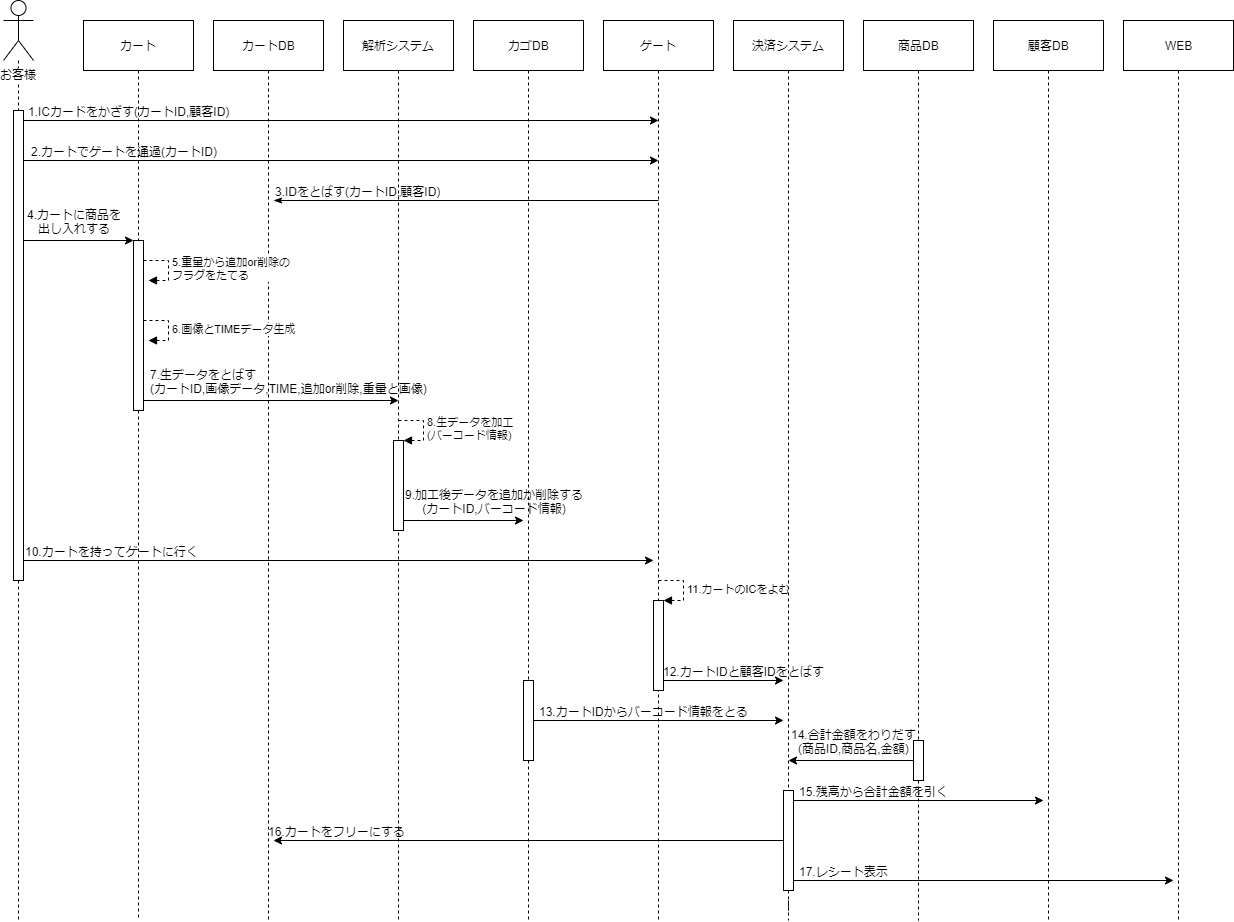
\includegraphics[width=15cm]{./picture/sequence_ic.eps}
\caption{ICタグを用いたシステムのシーケンス図}
\label{sequence_ic}
\end{figure}


以下の図\ref{sequence_qr}はQRコードを用いたシステムのシーケンス図である.


\begin{figure}[htbp]
\centering
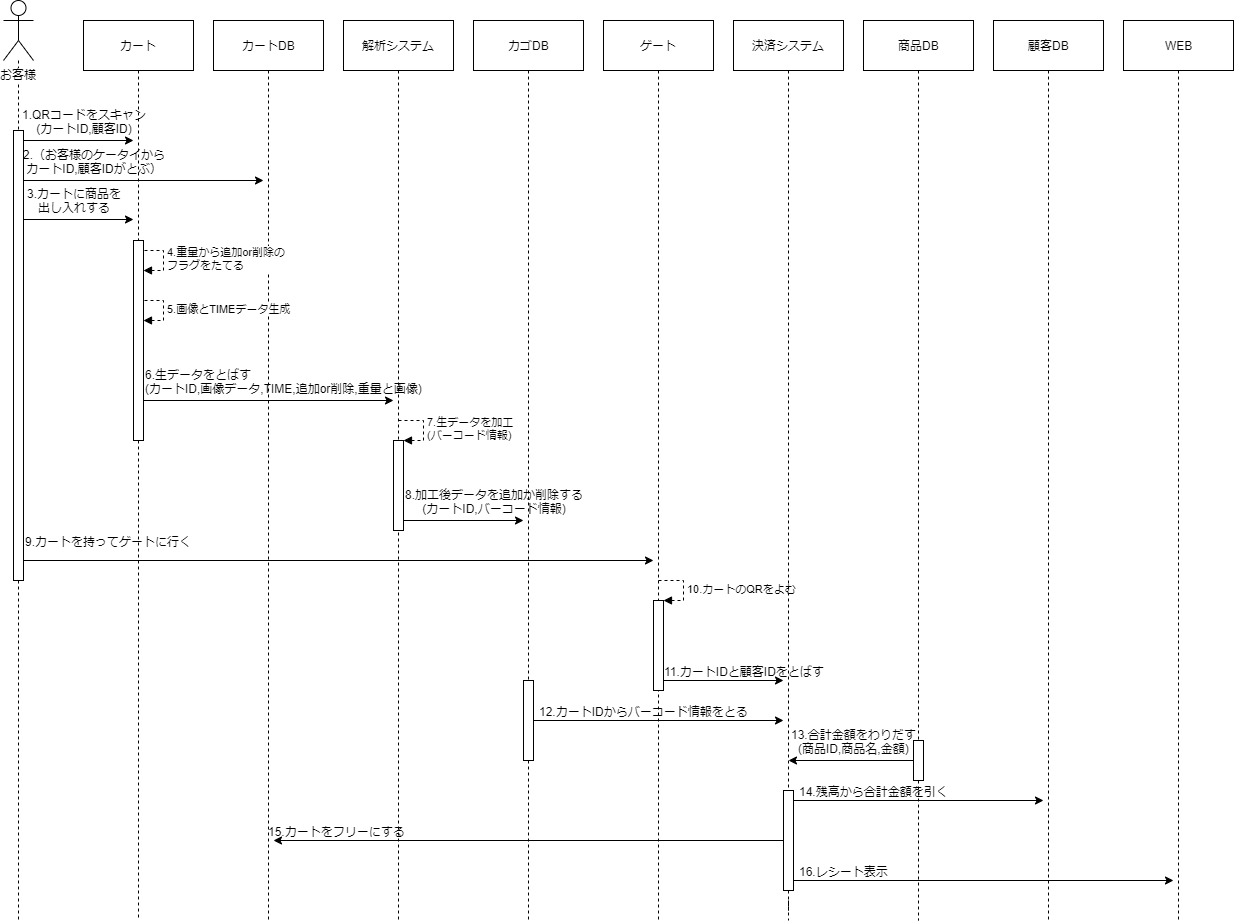
\includegraphics[width=15cm]{./picture/sequence_qr.eps}
\caption{QRコードを用いたシステムのシーケンス図}
\label{sequence_qr}
\end{figure}


本研究では,優先度の高いシステムである下記の図\ref{sequence}部分を実装する.


\begin{figure}[htbp]
\centering
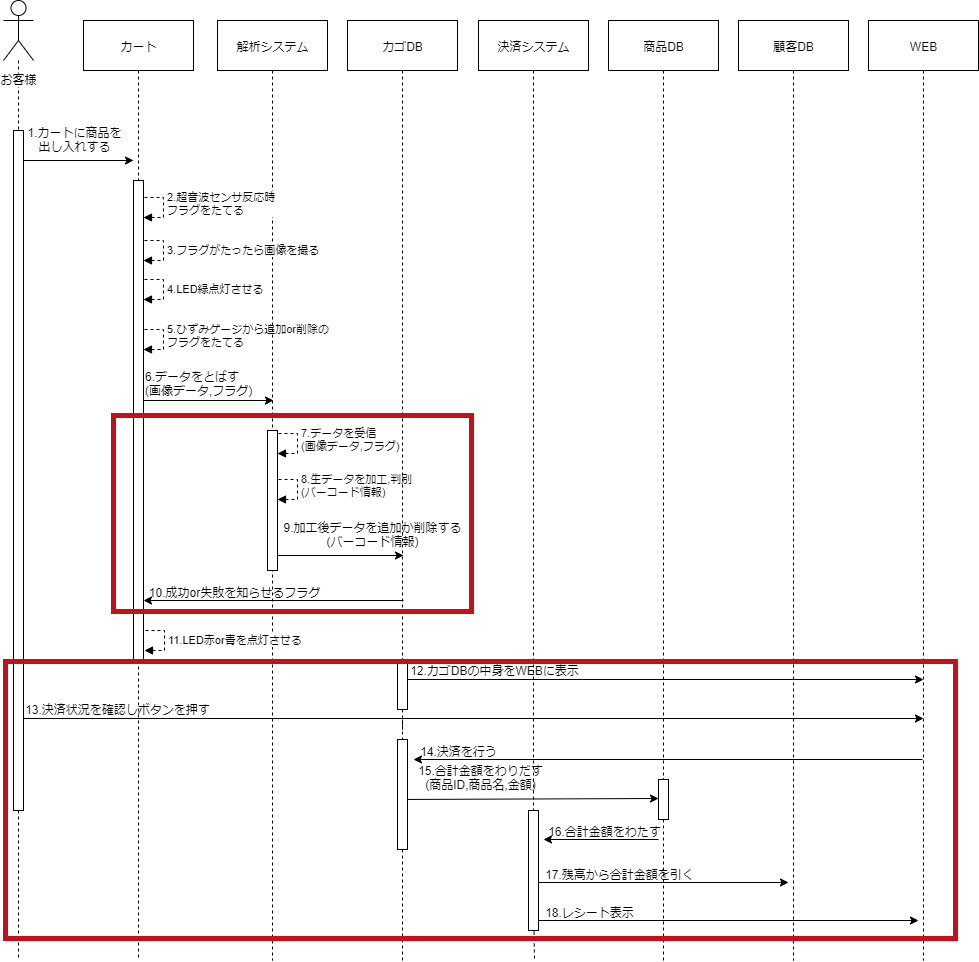
\includegraphics[width=15cm]{./picture/sequence.eps}
\caption{高優先度のシステムのシーケンス図}
\label{sequence}
\end{figure}